\section{Método de Monte Carlo}

Considere um círculo de raio $r=1$ inscrito em um quadrado de lado $2r$, como
mostra a Figura~\ref{fig:metodo}. Suas áreas são

\begin{equation}
    A_c = \pi r^2 = \pi
    \qquad\text{e}\qquad
    A_q = (2r)^2 = 4.
\end{equation}

\begin{figure}[H]
    \centering
    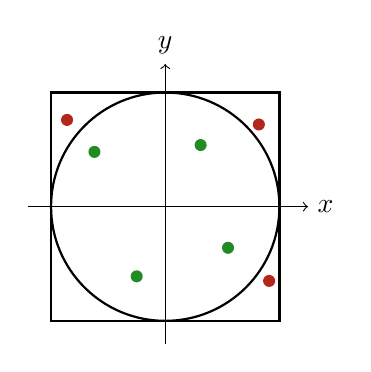
\begin{tikzpicture}[scale=1.45]
        \draw[thick] (-1,-1) rectangle (1,1);
        \draw[thick] (0,0) circle (1);
        \fill[ForestGreen] (-0.62,0.48) circle (1.5pt);
        \fill[ForestGreen] (0.31,0.54) circle (1.5pt);
        \fill[ForestGreen] (0.55,-0.36) circle (1.5pt);
        \fill[ForestGreen] (-0.25,-0.61) circle (1.5pt);
        \fill[BrickRed] (-0.86,0.76) circle (1.5pt);
        \fill[BrickRed] (0.82,0.72) circle (1.5pt);
        \fill[BrickRed] (0.91,-0.65) circle (1.5pt);
        \draw[->] (-1.2,0) -- (1.25,0) node[right] {$x$};
        \draw[->] (0,-1.2) -- (0,1.25) node[above] {$y$};
    \end{tikzpicture}
    \caption{Círculo unitário inscrito no quadrado de lado 2.}
    \label{fig:metodo}
\end{figure}

São sorteados $n$ pontos uniformes $(x,y)$ no quadrado. Um ponto pertence ao
círculo quando

\begin{equation}
    x^2+y^2 \leq 1.
\end{equation}

Se $d$ pontos estiverem dentro do círculo, a razão $d/n$ aproxima a razão
entre as áreas. Assim,

\begin{equation}
    \frac{d}{n}\approx\frac{A_c}{A_q}=\frac{\pi}{4}
    \quad\Longrightarrow\quad
    \pi\approx 4\frac{d}{n}.
\end{equation}

O erro é estatístico e tende a diminuir com o aumento de $n$, aproximadamente
na ordem de $1/\sqrt{n}$.
